\documentclass[a4paper,11pt]{article}
\input{/home/tof/Documents/Cozy/latex-include/preambule_lua.tex}
\newcommand{\showprof}{show them}  % comment this line if you don't want to see todo environment
\fancyhead[L]{Circuits combinatoires}
\newdate{madate}{10}{09}{2020}
\fancyhead[R]{Première - NSI} %\today
\fancyfoot[L]{~\\Christophe Viroulaud}
\fancyfoot[C]{\textbf{Page \thepage}}
\fancyfoot[R]{\includegraphics[width=2cm,align=t]{/home/tof/Documents/Cozy/latex-include/cc.png}}

\begin{document}
\begin{Form}
\section{Problématique}
Un ordinateur manipule des données codées sous forme de \emph{bits} en mémoire. Des combinaisons de transistors assurent des opérations booléennes élémentaires.
\begin{center}
\shadowbox{\parbox{14cm}{\centering À partir de ces éléments, comment réaliser une addition de nombres binaires?}}
\end{center}
\begin{commentprof}
Comment traduire le programme assembleur de l'addition (vu précédemment) en circuit électronique?
\end{commentprof}
\section{Fonctions logiques}
\subsection{Notations booléennes}
Les portes logiques évoquées dans les cours précédents peuvent être vues comme des fonctions booléennes élémentaires. On note ainsi les fonctions associées à chaque porte:
\begin{itemize}
\item $\lnot(x)$ pour NOT
\item $\land(x)$ pour AND
\item $\lor(x)$ pour OR
\end{itemize}
\subsection{Nouvelle porte logique}
Une porte logique élémentaire est également fréquemment utilisée dans les circuits électroniques: le \textbf{ou exclusif XOR}. Sa fonction booléenne associée se note $\oplus$.
\begin{commentprof}
fromage ou dessert
\end{commentprof}
\begin{table}[!h]
\begin{center}
\begin{tabular}{|c|c|c|}
\hline 
x & y & $x\oplus y$ \\ 
\hline 
0 & 0 & 0 \\ 
\hline 
0 & 1 & 1\\ 
\hline 
1 & 0 & 1\\
\hline 
1 & 1 & 0\\
\hline 
\end{tabular}
\caption{\label{xor}Fonction XOR}
\end{center}
\end{table} 
\begin{center}
\begin{tabular}{*{2}{>{\centering\arraybackslash}m{.4\textwidth}}}
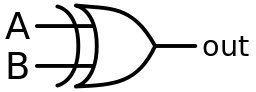
\includegraphics[width=4cm]{ressources/xor-us.png}
  & 
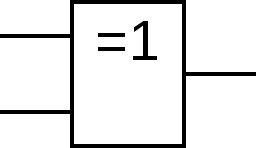
\includegraphics[width=3cm]{ressources/xor-eu.png}  
   \\
Symbole américain & Symbole européen
\end{tabular}
\end{center}
\subsection{Opérations booléennes}
Nous pouvons imaginer des fonctions booléennes complexes et déterminer leurs tables de vérités. Par exemple la fonction suivante \emph{f} et définit par:
$$f(x,y,z)=(x\land y)\oplus (\lnot y \lor z)$$
\begin{commentprof}
Nous pourrions écrire:
\begin{center}
(x AND y) XOR (NOT y OR z)
\end{center}
\end{commentprof}
\begin{activite}
\begin{enumerate}
\item La fonction \emph{f} a trois paramètres. Combien de combinaisons possibles peut-on réaliser avec ces paramètres?
\item Établir la table de vérité des différentes expressions ci-après (tableau \ref{expression}).
\item En déduire la table de vérité de~\emph{f} (tableau \ref{f}).
\end{enumerate}
\end{activite}

\begin{table}[!h]
\begin{center}
\begin{tabular}{|ccc|*4{c|}}
\hline 
x & y & z & $(x\land y)$ & $\lnot y$ & $(\lnot y \lor z)$\\ 
\hline 
0 & 0 & 0 &&&\\
\hline 
0 & 0 & 1 &&&\\
\hline 
... & ... & ... &&&\\
\hline 
\end{tabular}
\caption{\label{expression}Table de vérité de plusieurs expressions}
\end{center}
\end{table} 

\begin{table}[!h]
\begin{center}
\begin{tabular}{|ccc|c|}
\hline 
x & y & z & $(x\land y)\oplus (\lnot y \lor z)$\\ 
\hline 
0 & 0 & 0 &\\
\hline 
0 & 0 & 1 &\\
\hline 
... & ... & ... &\\
\hline 
\end{tabular}
\caption{\label{f}Table de vérité de \emph{f}}
\end{center}
\end{table} 
\section{Réaliser un additionneur}
\subsection{Décomposition}
Pour additionner deux nombres de \emph{n bits} il faut additionner bit à bit et prendre en compte une éventuelle retenue.\\
La première étape consiste à construire un additionneur 1 bit. Il est lui-même construit à partir de circuit plus simple: \emph{le demi-additionneur}.
\begin{commentprof}
Refaire un exemple d'addition
\end{commentprof}
\subsection{Demi-additionneur}
Un demi-additionneur prend deux bits en entrée $e_0$ et $e_1$ et renvoie la somme $e_0+e_1$ en sortie $s$. Il faut prendre en compte une éventuelle retenue $c$. La table de vérité correspondante est (Tableau \ref{demi}):
\begin{table}[!h]
\begin{center}
\begin{tabular}{|cc||cc|}
\hline 
$e_0$ & $e_1$ & s & c \\ 
\hline 
0 & 0 & 0 & 0 \\ 
\hline 
0 & 1 & 1 & 0\\ 
\hline 
1 & 0 & 1 & 0\\
\hline 
1 & 1 & 0 & 1\\
\hline 
\end{tabular}
\caption{\label{demi}Table de vérité du demi-additionneur}
\end{center}
\end{table} 
\begin{activite}
\begin{enumerate}
\item Quelles fonctions logiques reconnaît-on en \emph{s} et \emph{c}?
\item En déduire le schéma du demi-additionneur 1 bit.
\end{enumerate}
\end{activite}
\begin{commentprof}
\noindent$s=e_0\oplus e_1$\\
$c=e_0\land e_1$
\end{commentprof}
\subsection{Additionneur 1 bit}
Dans une addition bit à bit il faut prendre en compte l'éventuelle retenue de l'addition précédente. Ainsi un additionneur 1 bit prend trois entrées $e_0$, $e_1$ et la retenue précédente $c_0$. Il renvoie une sortie $s=e_0+e_1+c_0$ et une retenue éventuelle $c$.\\
En combinant deux demi-additionneurs nous pouvons construire un additionneur 1 bit.
\begin{activite}
\begin{enumerate}
\item Établir la table de vérité de l'additionneur 1 bit.
\item Sur la figure \ref{additionneur} placer les entrées $e_0$, $e_1$, $c_0$ et les sorties $s$ et $c$.
\end{enumerate}
\end{activite}
\begin{figure}[!h]
\centering
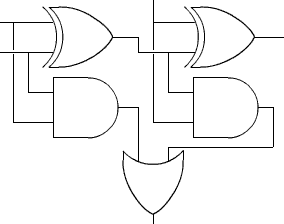
\includegraphics[width=5cm]{ressources/additionneur.png}
\captionof{figure}{Additionneur 1 bit}
\label{additionneur}
\end{figure}


\begin{commentprof}
logiciel logisim? \url{http://ww2.ac-poitiers.fr/techno-si/spip.php?article348}
\end{commentprof}
\end{Form}
\end{document}